\chapter{ハードウェア設計}
\label{cha:hardware_design}
\graphicspath{{figures/03_hardware_design}}


\section{システム構成}
\label{sec:hardware_overview}

システム構成は\ref{fig:hardware}です．
ああああああああああああああああああああああああああああああああああああああああああああああああああああああああああああああああああああああああああああああああああああああああああああああああああああああああああああああああああああああああああああああああああああああああああああああああああああああああああああああああああああああああああああああああああああああああああああああああああああああああああああ
\begin{figure}[htbp]
  \centering
  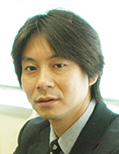
\includegraphics[width=0.3\linewidth]{ozaki.jpeg}
  \caption{システム構成}
  \label{fig:hardware}
\end{figure}


\section{機構設計}
\label{sec:mechanical_design}

移動機構とマニピュレータは\ref{fig:robot}です．
かかかかかかかかかかかかかかかかかかかかかかかかかかかかかかかかかかかかかかかかかかかかかかかかかかかかかかかかかかかかかかかかかかかかかかかかかかかかかかかかかかかかかかかかかかかかかかかかかかかかかかかかかかかかかかかかかかかかかかかかかかかかかかかかかかかかかかかかかかかかかかかかかかかかかかかかかかかかかかかかかかかかかかかかかかかかかかかかかかかかかかかかかかかかかかかかかかかかかかかかかかかかかかかかかかかかかかかかかかかかかか
\begin{figure}[htbp]
  \centering
  \begin{subfigure}[t]{0.3\textwidth}
    \centering
    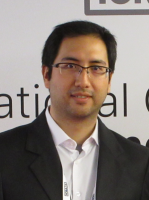
\includegraphics[width=\textwidth]{miyagusuku.png}
    \caption{移動機構}
    \label{fig:miyagusuku}
  \end{subfigure}
  \hfil
  \begin{subfigure}[t]{0.3\textwidth}
    \centering
    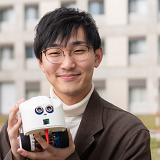
\includegraphics[width=\textwidth]{tabata.png}
    \caption{マニピュレータ}
    \label{fig:tabata}
  \end{subfigure}
  \caption{自律移動ロボット}
  \label{fig:robot}
\end{figure}

\subsection{移動機構の設計}
\ref{fig:miyagusuku}を説明します．
きききききききききききききききききききききききききききききききききききききききききききききききききききききききききききききききききききききききききききききききききききききききききききききききききききききききききききききききききききききききききききききききききききききききききききききききききききききききききききききききききききききききききききききききききききききききききききききききききききききききき

\subsection{マニピュレータの設計}
\ref{fig:tabata}を説明します．
くくくくくくくくくくくくくくくくくくくくくくくくくくくくくくくくくくくくくくくくくくくくくくくくくくくくくくくくくくくくくくくくくくくくくくくくくくくくくくくくくくくくくくくくくくくくくくくくくくくくくくくくくくくくくくくくくくくくくくくくくくくくくくくくくくくくくくくくくくくくくくくくくくくくくくくくくくくくくくくくくくくくくくくくくくくくくくくくくくくくくくくくくくくくくくくくくくくくくくくく

\chapter{Wi-FiとLiDARを用いた大域的自己位置推定}
\section{はじめに}
本章では，Wi-Fi尤度マップとLiDARによる大域的自己位置推定に関する手法を提案する．
まず，前章で述べたWi-Fi信号強度を格納した地図を基に，ロボット存在確率を表すWi-Fi尤度マップを構築し，このマップを用いた大域的自己位置推定を行う手法について説明する．
次に，Wi-Fi尤度マップの位置推定結果から，LiDARを用いてロボットの姿勢を推定する手法を述べる．
最後に，これらの手法を統合することで，大域的自己位置推定が可能であるか検証する．


\section{ハードウェア構成}
本研究で使用するハードウェア構成について説明する．
本研究で使用したロボットは，外形が全幅0.55[m]，全長0.72[m]，全高0.6[m]，全重量86[kg]の独立2輪駆動の車輪型ロボットである．
ロボットの前方には3D-LiDARが搭載しており，2次元スキャンデータを用いて幾何地図作成や自己位置推定を行った．
3章では，RS-LiDAR-32(Range: 0.4–200 [m])を用いて，4章では，VLP-16(Range: 0.5–100 [m])を用いて実験を行った．

\begin{table}[h]
 \begin{center}
 \caption{Robot specification}
  \begin{tabular}{|c||l|} \hline
    Robot name & Rebot \\ \hline \hline
    Size & Width = 0.55 [m] \\
    & Depth = 0.72 [m] \\
    &Height = 0.60 [m] \\ \hline
    Weight & 86.0 [kg] \\ \hline
    PC & Bord : AZW SER \\ 
     & CPU : Ryzen 5 5500u (AMD) \\
     & Mem : 16GB \\
     & OS : Ubuntu 22.04 LTS \\ \hline
    IMU & MPU9250 (TDK InvenSense) \\ \hline
    3D-LiDAR & RS-LiDAR-32 (robosense) ※Chapter 3 \\
             & VLP-16 (Velodyne Lidar) ※Chapter 4\\ \hline
    2D-LiDAR & RPLIDAR A2 $\times$2 (Slamtec) \\ \hline
    Wi-Fi antenna & Dual Band AC1200M Wi-Fi Adapter (Kangzio) $\times$8 \\ \hline
    Motor & BLH5100K-A (Oriental motor) \\ \hline
    Motor Driver and Encorder & BLVD20KM (Oriental motor) \\ \hline
    Battery & IFM24-400E2 $\times$2 (Kung Long Batteries) \\  \hline
   \end{tabular}
  \label{tab:spec_nict}
 \end{center}
\end{table}
\subsection{Wi-Fiセンサ}

このセンサーは無指向性であり，全方向からWi-Fi信号を受信できる．
\begin{figure}[h]
 \begin{minipage}{0.99\hsize}
  \begin{center}
   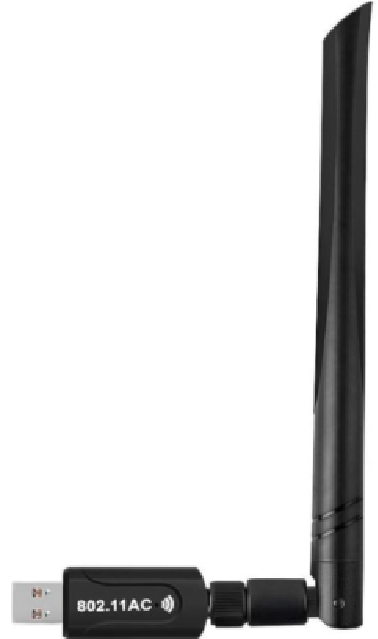
\includegraphics[scale=0.4]{figures/wifiantenna.pdf}
   \vspace{-3.0mm}
  \end{center}
   \vspace{-0.5mm}
  \caption{WiFi sensor}
  \label{fig:WiFi sensor}
  \end{minipage}
\end{figure}
\begin{table}[h]
 \begin{center}
 \caption{Specification of WiFi sensor}
  \begin{tabular}{|c||l|} \hline
    Standard & IEEE 802.11ac, IEEE 802.11n, IEEE 802.11g, IEEE 802.11b \\ \hline
    Interface & USB3.0\\ \hline
    Frequency Range & 2.4GHz ～ 2.4835GHz; 5.15GHz ～ 5.25GHz \\ \hline
    Wireless Speed & 11ac; up to 867Mbps \\
    & 11n; up to 300Mbps \\
    & 11g; 6/9/12/18/24/36/48/54 Mbps \\
    & 11b; 1/2/5.5/11 Mbps \\ \hline
    Working Channel Number & 1 ～ 14(2.4G); 36 ～ 165(5G) \\ \hline
    Spread Spectrum & DSSS \\ \hline
    Modulation Type & OFDM/CCK/16-QAM/64-QAM \\ \hline
    Wireless Transmit Power & 20dBm (MAX EIRP) \\ \hline
    Operate Environment & Operating Temperature: 0℃ ～ 40℃(32°F) \\ 
    & Storage Temperature: -40℃ ～ 70℃(-40°F) \\
    & Relative Humidity: 10\% ～ 90\%RH non-condensing \\
    & Storage Humidity: 5\% ～ 90\%RH non-condensing\\ \hline
   \end{tabular}
  \label{tab:spec_ant}
 \end{center}
\end{table}
\section{自己位置推定に用いる地図}
LiDARまたはWi-Fiを用いた自己位置推定を行うには，それぞれのセンサごとに対応した地図が必要となる．
本研究室におけるそれぞれの地図構築手法について説明する．
\subsection{幾何地図}
幾何地図の作成には，ROSのSLAMパッケージの一つであるgmappingを使用した．
gmappingは，オドメトリデータとLiDARの2次元スキャンデータを用いて地図を作成するパッケージである．
本論文では，LiDARにより取得した2Dスキャンデータと，エンコーダとIMUデータから算出したオドメトリ情報を入力として地図を作成した．
gmappingにより生成される地図は，障害物があるグリッドを黒(0)，障害物がないグリッドを白(255)，未知の領域を灰色(127)の値で出力される．

本研究室で使用するLiDARによる自己位置推定では，幾何地図として占有格子地図を用いるため，gmappingで生成した地図を各格子ごとに障害物の存在確率を表した地図に変換する必要がある．
ここで，地図の中で障害物を占有しているグリッド間のユーグリッド距離$\displaystyle dist$を定義したとき，地図上で占有される確率を平均ゼロのガウス分布で以下の式により表す(3.1)．

\begin{equation}
\displaystyle m_{u,v}=z_{hit}exp\left(\frac{dist^{2}}{2\sigma ^{2}}\right)+( 1-z_{hit})
\end{equation}
ここで，$\displaystyle z_{hit}$はガウス分布によるLiDARの重みを表し，観測のノイズや外れ値を考慮するためのパラメータである．
また$\displaystyle m_{u,v}$は地図上の位置$\displaystyle u$，$\displaystyle v$における地図の占有確率を示す．
$\displaystyle \sigma $はガウス分布の分散であり，占有の広がりを決定する要因である．
% gmappingによる地図と占有格子地図に変換した地図を{\bf Fig.}~\ref{fig:gridmap}，{\bf Fig.}~\ref{fig:geomap}に示した．
グリッドサイズは0.2[m]とした．
\begin{figure}[h]
 \begin{minipage}{0.49\hsize}
  \begin{center}
   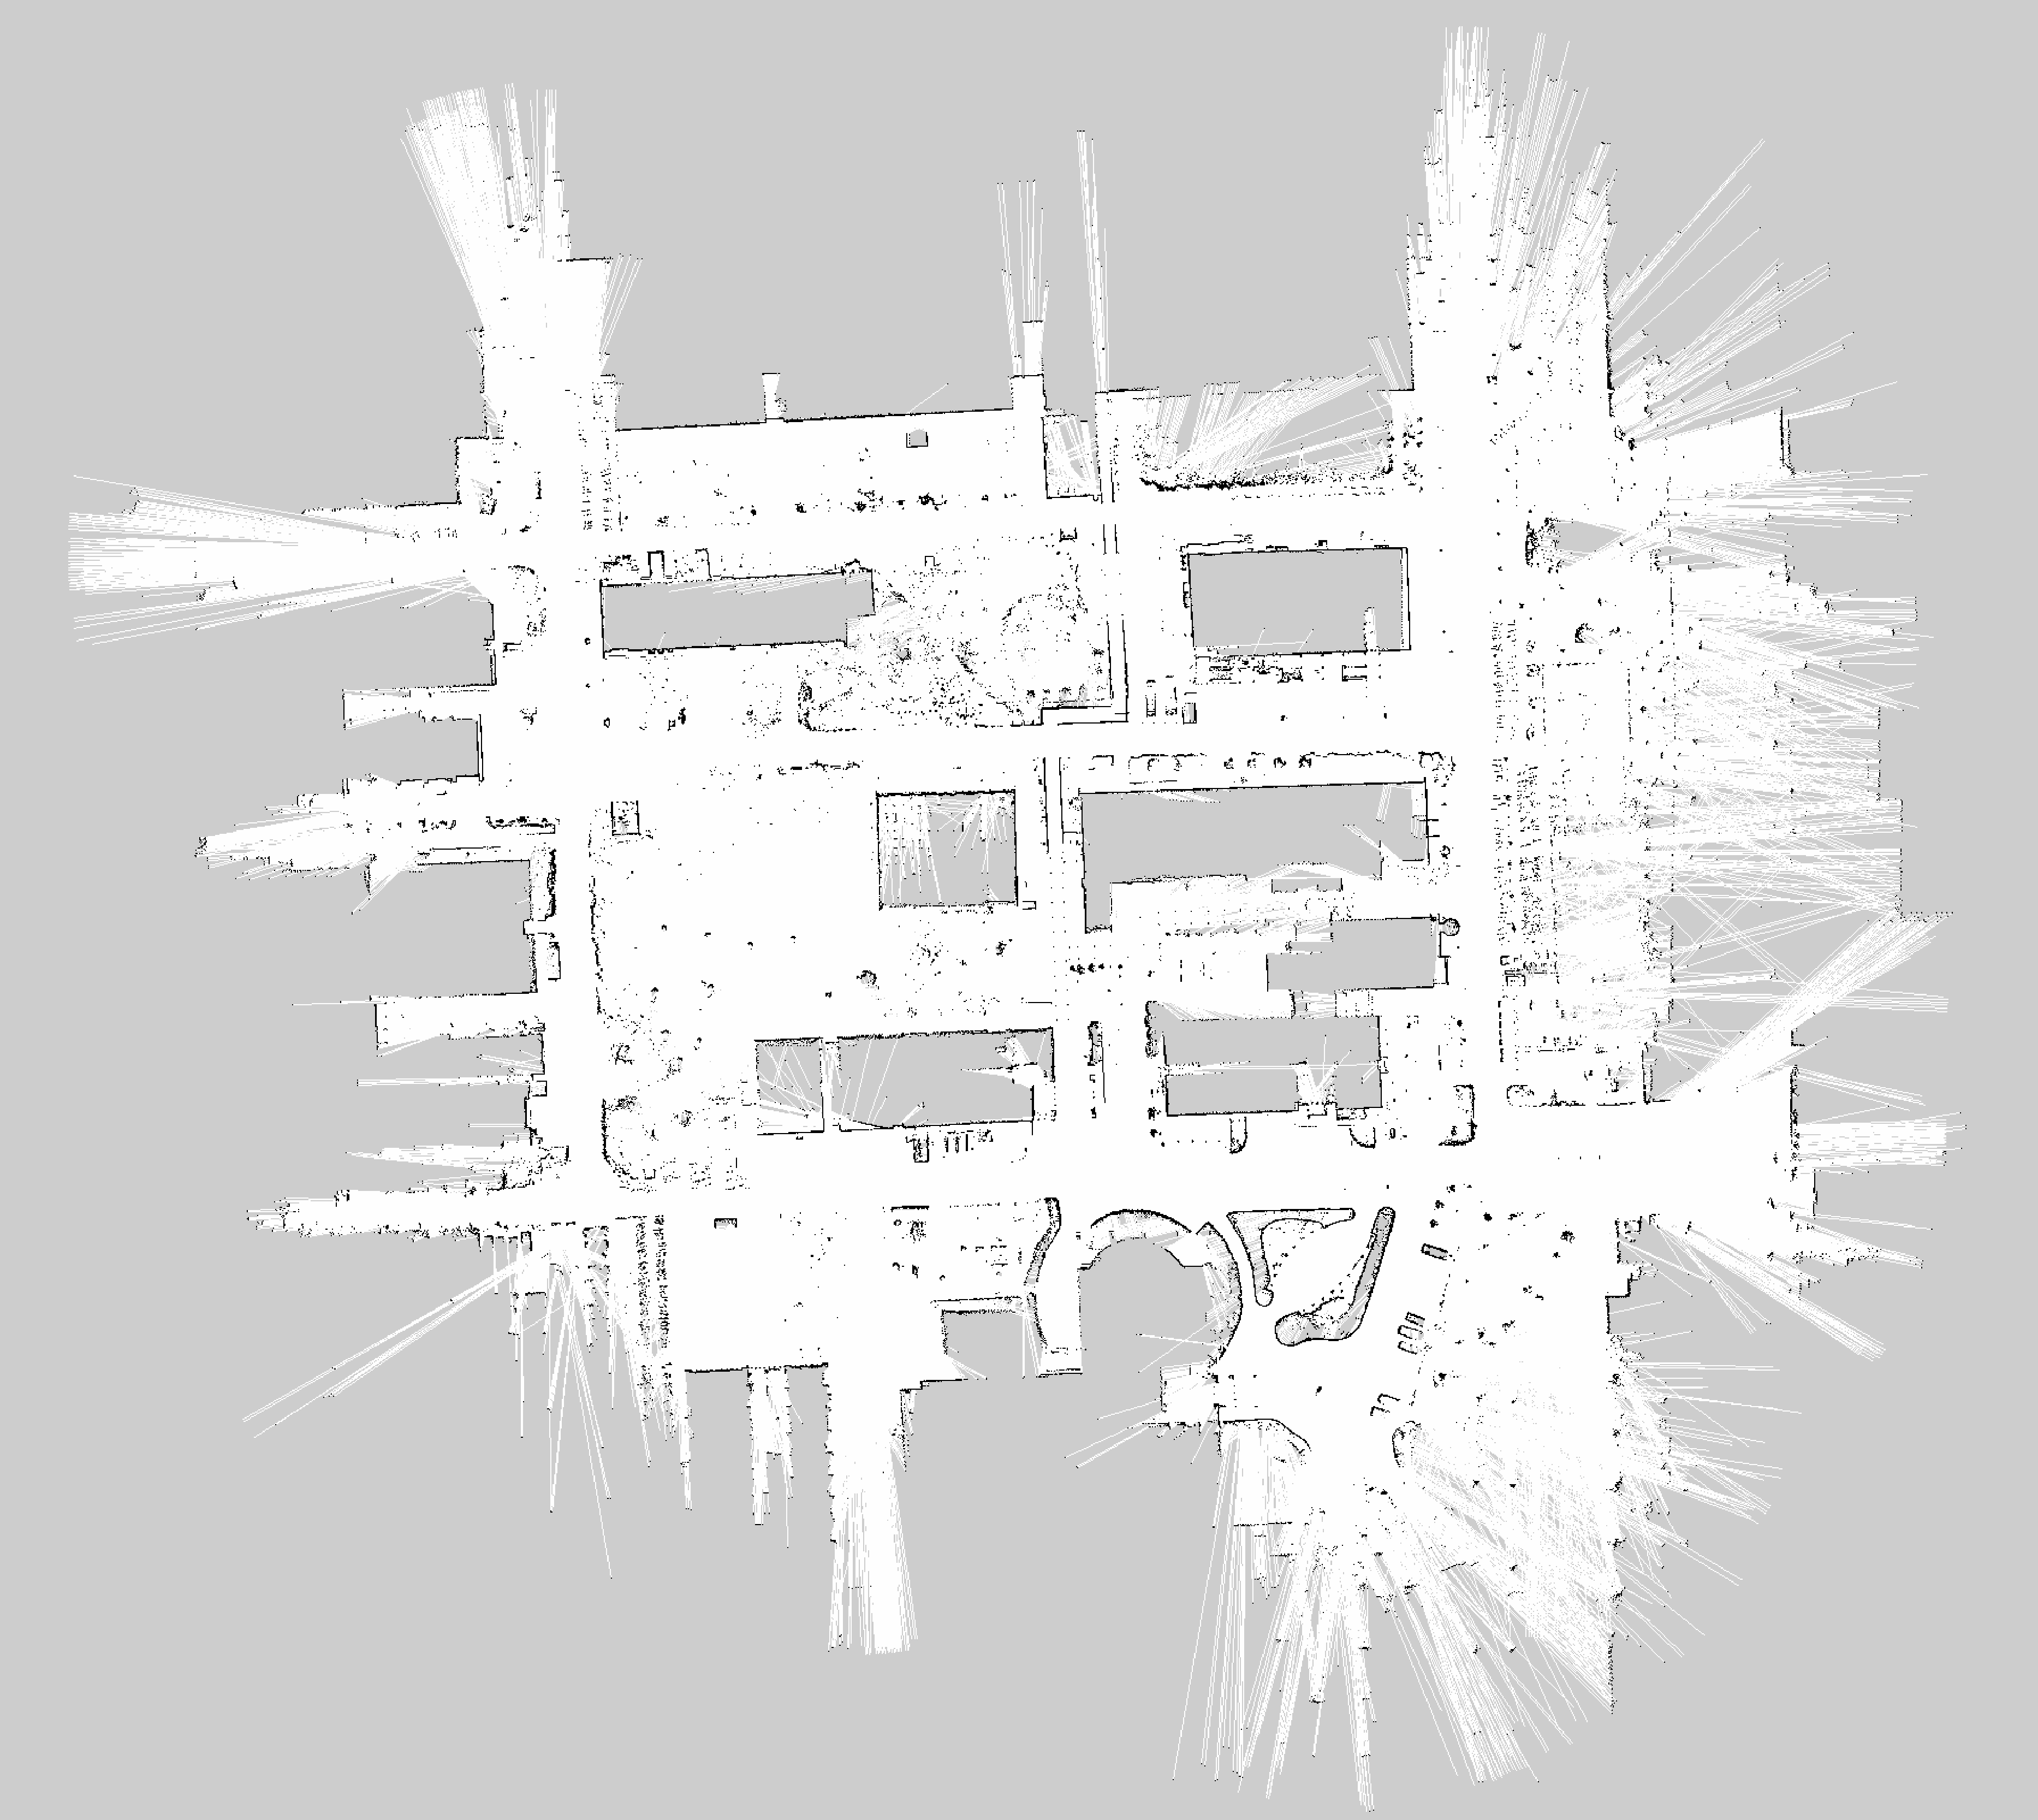
\includegraphics[scale=0.1]{figures/map.pdf}
   \vspace{-3.0mm}
  \end{center}
   \vspace{-0.5mm}
  \caption{Geometric map created by gmapping}
  \label{fig:gridmap}
  \end{minipage}
 \begin{minipage}{0.49\hsize}
  \begin{center}
   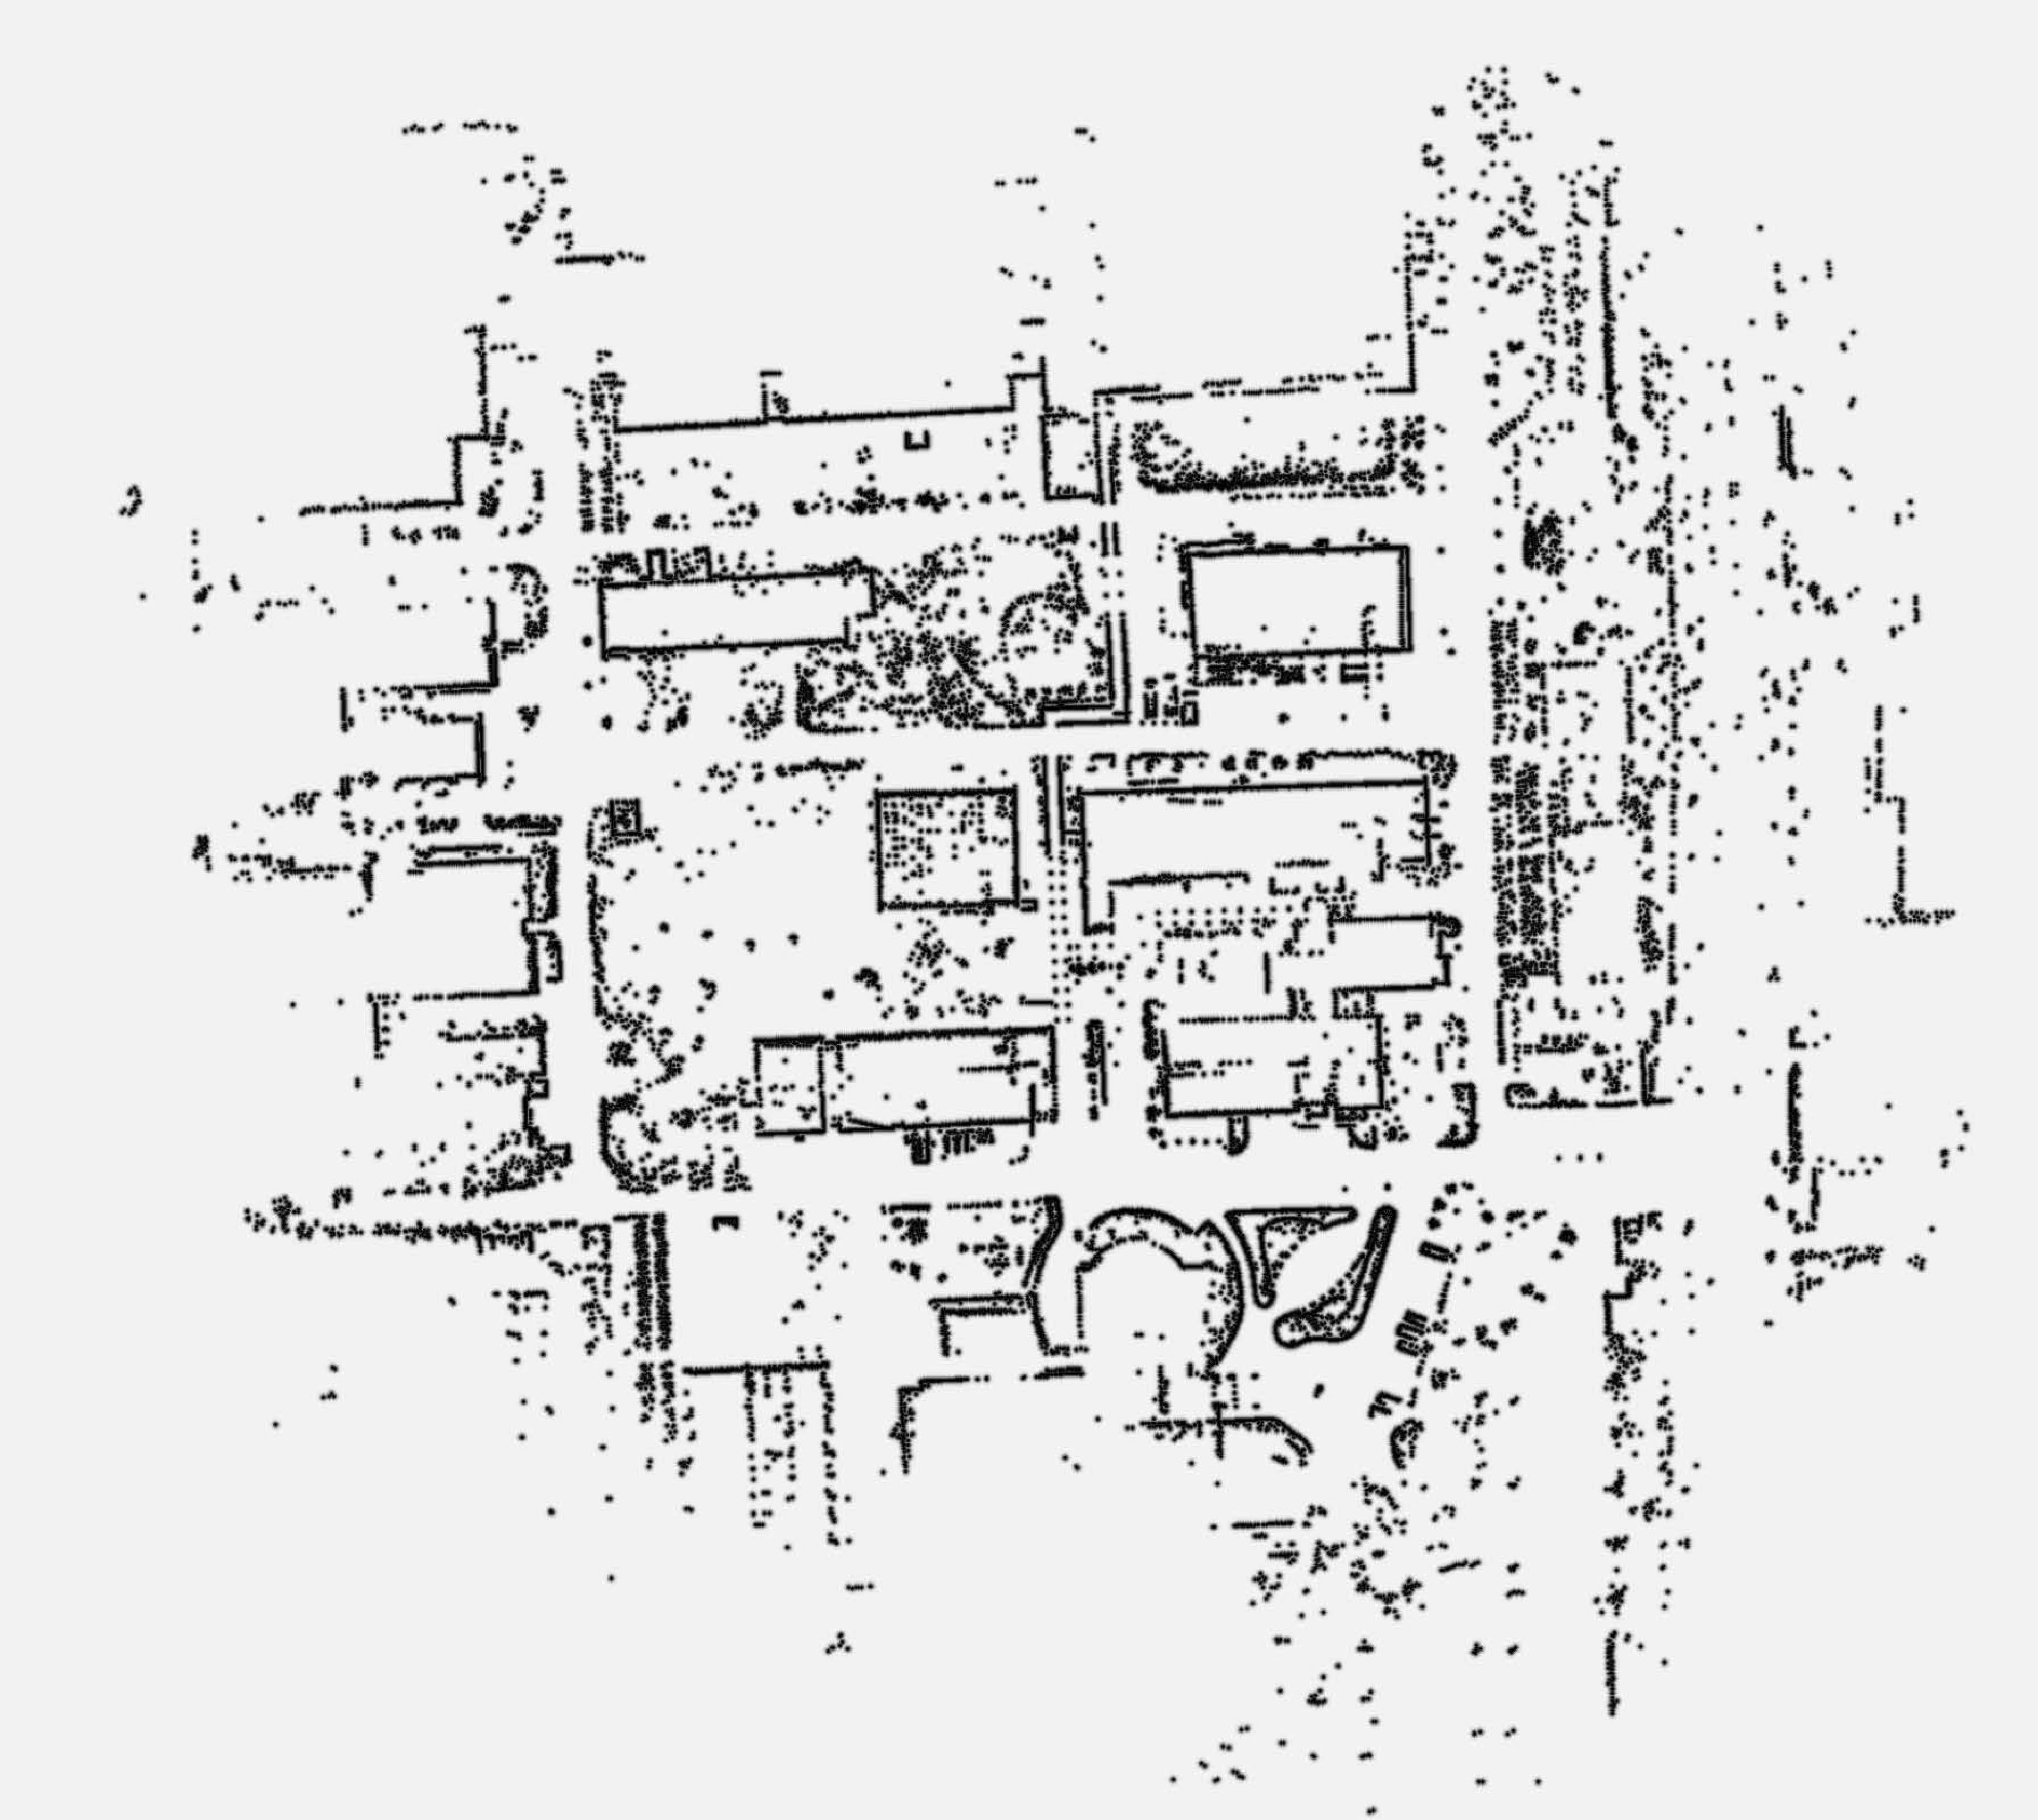
\includegraphics[scale=0.1]{figures/12zemi.pdf}
   \vspace{-3.0mm}
  \end{center}
   \vspace{-0.5mm}
  \caption{Map converted from geometric map to occupied grid map}
  \label{fig:geomap}
  \end{minipage}
\end{figure}
\subsection{Wi-Fi地図}
Wi-Fi地図の地図構築に必要なステップは下記の通りである．
\subsection*{1. データ取得}
ロボットを手動走行させ，オドメトリ，LiDARのスキャンデータ，Wi-Fi信号強度を記録する．
次にオドメトリ，LiDARのスキャンデータから先ほどのgmappingを用いて幾何地図を作成する．
幾何地図作成後，rosのAMCLから幾何地図を作成した際のデータを用いて自己位置推定を行う．
その自己位置推定結果$\displaystyle \mathbf{x} =( x,y,\theta )$と,Wi-Fi信号強度の観測値$\displaystyle \mathbf{z}$に対応付けたデータセットを作成する．
ただし，$\displaystyle \mathbf{z}$は，位置$\displaystyle \mathbf{x}$で観測できた異なる$\displaystyle m$個のAPの信号強度を並べたベクトル$\displaystyle \mathbf{z} =[ z_{1} ,z_{2} ,...,z_{m}]$である．

この際，各マックアドレスのWi-Fiの信号強度は3秒間に観測されたデータの平均値とした．
また，5か所以上でWi-Fiの信号強度を観測できたAPのみを使用した．
これはモバイルAPを含まないようにするためである．
ただしこれらの数値は，Wi-Fiの信号強度のノイズや減衰の状況などを考慮して決定したものではないため，より適切な数値の選択のための手法構築は今後の課題である．
\subsection*{2. ガウス回帰過程}
ロボットがデータ取得時に走行した経路上のみWi-Fi信号強度のデータが存在し，走行経路以外ではデータがないため，自己位置推定が不可能である．
したがって，任意の経路で自己位置推定を行うためには，走行経路全域のWi-Fi信号強度を格納した地図が必要となる．
そこで本研究室では，ガウス過程回帰(GPR:Gaussian Process Regression)を用いて，データセットをもとに走行経路外のWi-Fiの信号強度を補完することで，走行環境全域の信号強度の分布を予測した\cite{miyagusuku2018precise}．
\subsection*{3. Wi-Fi地図作成}
ガウス過程回帰により取得した分布をもとに，指定した解像度の格子にデータを格納することで，最終的なWi-Fi信号強度を用いた自己位置推定に用いる地図が完成する．
予測値の平均値は各APごとに行われ，分散は全てのAPに共通するため，Wi-Fi地図はアクセスポイント数枚，分散地図は一枚となる．
グリッドサイズは1[m]とした．
\begin{figure}[h]
 \begin{minipage}{0.99\hsize}
  \begin{center}
   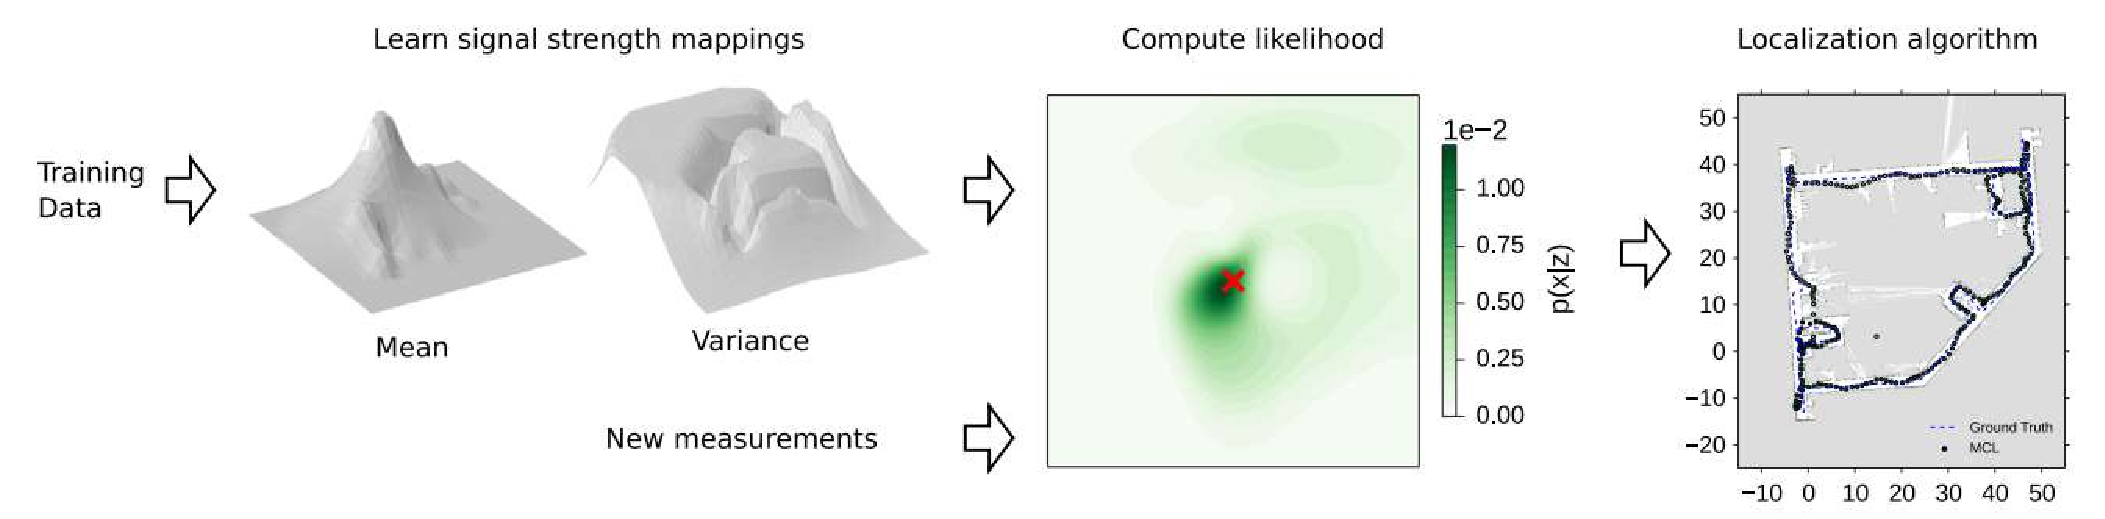
\includegraphics[scale=0.4]{figures/gprwifi.pdf}
   \vspace{-3.0mm}
  \end{center}
   \vspace{-0.5mm}
  \caption{Overview of wireless-based localization using signal strength mapping\cite{miyagusuku2018precise}}
  \label{fig:gprwifi}
  \end{minipage}
\end{figure}
\section{LiDARを用いた局所的自己位置推定}
本研究室のLiDARを用いた自己位置推定はDellaertらによって提案されたMCL\cite{mcl}がベースとなっている．
MCLとは，ロボットを疑似に表現したパーティクルと呼ばれる粒子を用いることで，ロボットの存在確率を表現する手法である．
位置推定のプロセスは以下の通りである．
まず，ロボットの初期位置付近にパーティクルをサンプリングする．
ここで，各パーティクルはロボットの状態の一つの候補を表す．
次に，ロボットが移動した際，内界センサによる移動量から動作モデルに従ってパーティクルの状態が更新される．
その後に，ロボットが外界センサにより観測されたセンサデータを各パーティクルに与える．
ここで，パーティクルが観測するであろうセンサデータと実際に観測したセンサデータとの比較を行い，一致している度合いに応じて各パーティクルに尤度を与える．
この尤度が大きいほどロボットの状態に近いとされ，ロボットの位置推定に利用される．
さらに，パーティクルの尤度の偏りを検知するEffective Sample Size(ESS)\cite{ess}を用いることで，全パーティクルの中で自己位置推定に有効なパーティクルの個数を検知する．
このESSが一定の閾値を下回った場合にパーティクルにリサンプリングを行う．
このとき，尤度の小さいパーティクルは削除され，尤度の高いパーティクルにサンプリングされる．
以上のプロセスを一度行うと，自己位置推定が1ステップ実行されたことになる．
ロボットはこのプロセスを繰り返すことで，自己位置を確信する．
パーティクルは確率分布に基づいてサンプリングされるため，ミスマッチングによるパーティクルの収束を防げる可能性がある．
そのため，ロバストな自己位置推定の実現が可能になる．
パーティクル数が増加すれば，それに伴ってロボットの存在確率をより近似できるためロバスト性が向上する．
しかし，パーティクルの個数が多すぎると情報量も増加するため，計算コストが高くなってしまい，リアルタイムに位置推定が行えなくなるといった課題もある．
以下に本手法の位置推定の流れを示す．

\subsection{動作モデルに基づいたパーティクルの更新}
動作モデルを考える時，時刻$\displaystyle t-1$の時点でパーティクルが与えられていると仮定する．
ロボットは車輪の回転量から時刻$\displaystyle t-1$から時刻$\displaystyle t$の間の移動量を計測することができる．
この移動量を用いて，ロボットの動作モデルに従って状態を更新すると，時刻$\displaystyle t$における事前分布を予測できる．
この予測をオドメトリと呼び，車輪型移動ロボットにおいて，広く用いられる\cite{fox2005probabilistic}．
以下でオドメトリによる動作モデルについて説明をする．

本研究で対象とする車輪型ロボットは，二次元平面上でのみを移動すると仮定する．
% このときロボットの位置は{\bf Fig.}~\ref{fig:robotpose}に示す座標系において，
\begin{equation}
    \mathbf{x} 
    =
    \begin{pmatrix}
        x \\ y \\ \theta
    \end{pmatrix}
\end{equation}
で表現される．
また，ロボットの前回$\displaystyle \mathbf{x}$$\displaystyle _{t-1}$と現在の状態$\displaystyle \mathbf{x}$$\displaystyle _{t}$までの動作を表す３つのパラメータ$\displaystyle \hat{\delta }_{rot1}$，$\displaystyle \hat{\delta }_{trans}$，$\displaystyle \hat{\delta }_{rot2}$を次のように定める．
\begin{equation}
\displaystyle \hat{\delta }_{rot1} =\delta _{rot1} +\varepsilon _{\alpha 1} \delta _{rot1} +\alpha _{2} \delta _{trans}
\end{equation}
\begin{equation}
\displaystyle \hat{\delta }_{trans} =\delta _{trans} +\varepsilon _{\alpha 3} \delta _{trans} +\alpha _{4} \delta _{rot1} +\alpha _{4} \delta _{rot2}  
\end{equation}
\begin{equation}
\displaystyle \hat{\delta }_{rot2} =\delta _{rot2} +\varepsilon _{\alpha 1} \delta _{rot2} +\alpha _{2} \delta _{trans}
\end{equation}
ここで，$\displaystyle \varepsilon _{b}$は平均0，$\displaystyle b$の正規分布に従う値とし，式(3.3)～式(3.5)内に$\displaystyle b$の実体として付されている$\displaystyle \alpha _{1}～\displaystyle \alpha _{4}$はロボット固有のノイズパラメータである．
走行距離ノイズを$\sigma_\text{dist}$，角度ノイズを$\sigma_\text{angle}$として，これらのノイズパラメータを以下のように定義する．
\begin{description}
    \item[\hspace{2em}]  $\alpha_1$：回転運動による回転誤差 $\alpha_1=\sigma_\text{angle}$
    \item[\hspace{2em}]  $\alpha_2$：並進運動による回転誤差 $\alpha_2=\sigma_\text{angle} \times \sigma_\text{dist}$
    \item[\hspace{2em}]  $\alpha_3$：並進運動による並進誤差 $\alpha_3=\sigma_\text{dist}$
    \item[\hspace{2em}]  $\alpha_4$：回転運動による並進誤差 $\alpha_4=\sigma_\text{dist} \times \sigma_\text{angle}$
\end{description}
以上より，$\displaystyle \hat{\delta }_{rot1}$，$\displaystyle \hat{\delta }_{trans}$，$\displaystyle \hat{\delta }_{rot2}$を用いたオドメトリ動作モデルは，次式として表現できる．
\begin{equation}
\begin{pmatrix}
x_{t+1} \\ 
y_{t+1} \\ 
\theta_{t+1}
\end{pmatrix}
=
\begin{pmatrix}
x_{t} \\ 
y_{t} \\ 
\theta_{t}
\end{pmatrix}
+
\begin{pmatrix}
\displaystyle \hat{\delta }_{trans} \cos( \theta _{t} +\hat{\delta }_{rot1}) \\ 
\displaystyle \hat{\delta }_{trans} \sin( \theta _{t} +\hat{\delta }_{rot1}) \\ 
\displaystyle \theta _{t} +$$\displaystyle \hat{\delta }_{rot1}$$\displaystyle +\hat{\delta }_{rot2}
\end{pmatrix}
\end{equation}
これにより，パーティクルが移動の不確かさを表現することにより，パーティクルの分布が拡張して遷移していく．
% パーティクルの状態更新に用いる動作モデルは{\bf Fig.}~\ref{fig:odommodel}に示す．



\begin{figure}[t]
 \begin{minipage}{0.99\hsize}
  \begin{center}
   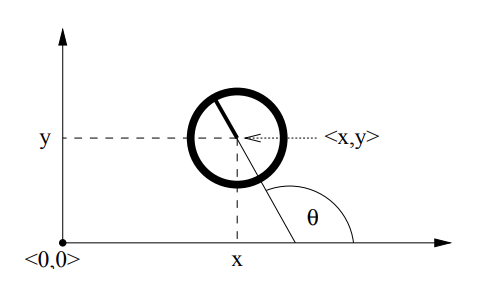
\includegraphics[scale=0.6]{figures/poseinglobalcoord.png}
   \vspace{-3.0mm}
  \end{center}
   \vspace{-0.5mm}
  \caption{Robot Pose Shown in a Global Coordinate System\cite{fox2005probabilistic}}
  \label{fig:robotpose}
  \end{minipage}
\end{figure}

\begin{figure}[h]
 \begin{minipage}{0.99\hsize}
  \begin{center}
   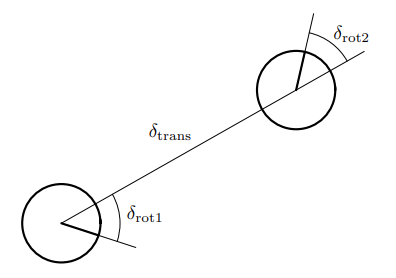
\includegraphics[scale=0.6]{figures/odommodel.png}
   \vspace{-3.0mm}
  \end{center}
   \vspace{-0.5mm}
  \caption{Odometry model: The robot motion in the time interval$\displaystyle (t-1, t)$ is
approximated by a rotation $\displaystyle \delta_{rot1}$, followed by a translation $\displaystyle \delta_{trans}$ and a
second rotation $\displaystyle \delta_{rot2}$. The turns and translation are noisy\cite{fox2005probabilistic}.}
  \label{fig:odommodel}
  \end{minipage}
\end{figure}

\subsection{尤度計算}
尤度計算は，動作モデルにより予測された各パーティクルの尤もらしさを算出するステップである．
尤もらしさとは確率に似た概念であるが，確率の定義である和が1になるという制約を満たさないため，確率とは別の呼び方をしている．

本研究室では，幾何地図として占有格子地図を用いる．
占有格子地図は255階調のグレースケールのグリッドマップで表現している．
そのため，観測の独立性を仮定することで，パーティクルの尤度$\displaystyle \omega $を次のように求める．
\begin{equation}
\displaystyle \omega _{i} =\frac{m_{u,v}}{b} 
\end{equation}
\begin{equation}
\displaystyle \omega =exp\left\{\frac{1}{N}\sum _{i=1}^{N}( log\ \omega _{i})\right\}
\end{equation}

ここで，LiDARのスキャンデータの位置$\displaystyle u$，$\displaystyle v$における地図の占有確率を$\displaystyle m_{u,v}$，LiDARのレーザ1本に対する尤度を$\displaystyle \omega _{i}$，LiDARの1回のスキャンで観測したレーザの本数を$\displaystyle N$，輝度の最大値を$\displaystyle b$とする\cite{onolidar}．
この尤度計算は地図に表現されている情報を尤度として捉えて設計された尤度関数である．
この尤度関数は他のLiDARの尤度関数に比べて計算コストが低いため，リアルタイムな位置推定が求められるロボットの尤度計算に適している．
しかし，計測値を短くする原因となる動的障害物の影響を考慮した設計とはなっていないため，より動的障害物に強い手法の構築は今後の課題である．
\subsection{位置推定}
MCLはロボットの位置を確率分布として表現するフレームワークであるが，ロボットのナビゲーションのためには確率分布ではなく，1点の代表点を計算する必要がある．
代表点の計算手法として，最尤値計算と重み付け平均の2種類あるが，本論文では重み付け平均を採用する．
したがって，式(3.9)に従って時刻$\displaystyle t$におけるロボットの推定結果とする．
$\displaystyle j$はある地点でのパーティクルで，$\displaystyle n$はパーティクル数を表している．
\begin{equation}
 \displaystyle \mathbf{x}_{t} =\sum _{j=1}^{n} \omega _{t}^{j} x_{t}^{j} 
\end{equation}
\subsection{パーティクルのリサンプリング}
MCLでは3.4.1節で説明した通り，1ステップ移動するたびにノイズをモデル化した確率分布からパーティクルをサンプリングするため，パーティクルによってはロボットの真の状態と大きく異なっている可能性がある．
この場合，予測された確率分布は広がり続けてしまい位置推定性能が低下する．
したがって，不要なパーティクルは削除し，真の状態に近い場所にサンプリングし直すことで，より精密かつ正確な確率分布を生成したい．
このときパーティクルをサンプリングし直すことをリサンプリングとよぶ．
リサンプリングは，パーティクルの重みに偏りが現れた際にのみに行う方が効率がよい．
尤度の偏り検知には式(3.10)により計算されるESSを用いた．
これは全パーティクルの中で自己位置推定に有効なパーティクルの個数を検知する．
このESSが一定の閾値を下回ったときパーティクルのリサンプリングを行う．
\begin{equation}
 \displaystyle \eta _{ess} =\frac{1}{\sum _{j=1}^{n} \omega _{j}^{2}}   
\end{equation}
